% Module 4: Robotics - short assignment report
% Compile with XeLaTeX: latexmk -xelatex report.tex
\documentclass{article}

\PassOptionsToPackage{numbers,compress}{natbib}
\usepackage[final]{template22}
% Common packages
\usepackage[utf8]{inputenc} % allow utf-8 input
\usepackage[T1]{fontenc}    % use 8-bit T1 fonts
\usepackage{microtype}
\usepackage{times}
\usepackage{graphicx}
\usepackage{amsmath,amssymb,mathbbol}
% \usepackage{algorithmic}
% \usepackage[linesnumbered,ruled,vlined]{algorithm2e}
\usepackage{acronym}
\usepackage{enumitem}
\usepackage[pagebackref=true,breaklinks=true,colorlinks]{hyperref}
\usepackage{balance}
\usepackage{xspace}
\usepackage{setspace}
\usepackage[skip=3pt,font=small]{subcaption}
\usepackage[skip=3pt,font=small]{caption}
\usepackage[dvipsnames]{xcolor}
\usepackage[capitalise]{cleveref}
\usepackage{booktabs,tabularx,colortbl,multirow,array,makecell}
% \usepackage{overpic,wrapfig}

\usepackage{fancyhdr}
\hypersetup{pdfencoding=auto,colorlinks=true,allcolors=black}
\renewcommand{\headrulewidth}{0.5pt}
\renewcommand{\footrulewidth}{0pt}
\fancyhf{}
\fancyhead[C]{}
\fancyhead[C]{}
\fancyfoot[C]{\thepage}

% Handy shorthand
\makeatletter
\DeclareRobustCommand\onedot{\futurelet\@let@token\@onedot}
\def\@onedot{\ifx\@let@token.\else.\null\fi\xspace}
\def\eg{\emph{e.g}\onedot} 
\def\Eg{\emph{E.g}\onedot}
\def\ie{\emph{i.e}\onedot} 
\def\Ie{\emph{I.e}\onedot}
\def\cf{\emph{c.f}\onedot} 
\def\Cf{\emph{C.f}\onedot}
\def\etc{\emph{etc}\onedot} 
\def\vs{\emph{vs}\onedot}
\def\wrt{w.r.t\onedot} 
\def\dof{d.o.f\onedot}
\def\etal{\emph{et al}\onedot}
\makeatother

\definecolor{gray}{gray}{0.9}

% Handy math ops
\DeclareMathOperator*{\argmax}{arg\,max}
\DeclareMathOperator*{\argmin}{arg\,min}
\newcommand{\norm}[1]{\left\Vert #1 \right\Vert}

% % Spacing
\frenchspacing
% \medmuskip=2mu   % reduce spacing around binary operators
% \thickmuskip=3mu % reduce spacing around relational operators
% \setlength{\abovedisplayskip}{3pt}
% \setlength{\belowdisplayskip}{3pt}
% \setlength{\abovecaptionskip}{3pt}
% \setlength{\belowcaptionskip}{3pt}
\setlength\floatsep{0.5\baselineskip plus 3pt minus 2pt}
\setlength\textfloatsep{0.5\baselineskip plus 3pt minus 2pt}
\setlength\dbltextfloatsep{0.5\baselineskip plus 3pt minus 2pt}
\setlength\intextsep{0.5\baselineskip plus 3pt minus 2pt}

\makeatletter
\renewcommand{\paragraph}{%
  \@startsection{paragraph}{4}%
  {\z@}{0ex \@plus 0ex \@minus 0ex}{-1em}%
  {\hskip\parindent\normalfont\normalsize\bfseries}%
}
\makeatother

% Graphics path
\graphicspath{{figures/}}

% Clever references
\crefname{algorithm}{Alg.}{Algs.}
\Crefname{algorithm}{Algorithm}{Algorithms}
\crefname{section}{Sec.}{Secs.}
\Crefname{section}{Section}{Sections}
\crefname{table}{Tab.}{Tabs.}
\Crefname{table}{Table}{Tables}
\crefname{figure}{Fig.}{Fig.}
\Crefname{figure}{Figure}{Figure}

% Acronym
\acrodef{pku}[PKU]{Peking University}
\usepackage{tikz}
\usetikzlibrary{arrows.meta,positioning,shapes.geometric}
\usepackage{algorithm}
\usepackage{algorithmic}

\title{Closed-Loop Robotic Block Stacking:\\
Motion Planning, Collision-Aware Grasping, and Depth-Camera Perception}

\author{%
  Yuanze Lei \quad 2510124204\\
  Peking University
}

\begin{document}
\maketitle

\begin{abstract}
This report presents a design for a robot that stacks a set of blocks whose poses
and extents are known. The task is formulated with rigid-body transforms, a
stable placement order, top grasps, and collision-aware motion planning. We show
how the grasp, pre-grasp, lift, and place poses are computed and identify the
arguments that must be supplied to a planner. A vertical pre-grasp and a
short Cartesian descent avoid the common failure mode in which the gripper
collides with the target block. We then relax the known-pose assumption and
describe an RGB-D pipeline for calibration, segmentation, pose estimation, scene
updating, execution, and recovery. The report makes no experimental claims: it
specifies an implementable procedure and explains the role of each module.
\end{abstract}

\section{Problem Formulation}\label{sec:problem}

We consider a robot arm, a table, and $N$ rigid blocks. Let
$\mathbf{q}\in\mathbb{R}^{n}$ denote the vector of joint positions for an
$n$-degree-of-freedom arm. The base of the robot is frame $B$, and frame $G$
is attached to the tool centre point (TCP) of the parallel-jaw gripper. Every
block $i$ has a centre frame $O_i$, dimensions $(w_i,d_i,h_i)$, and a known pose
$\mathbf{T}_{B\leftarrow O_i}\in SE(3)$. The notation
$\mathbf{T}_{A\leftarrow C}$ means that a point expressed in frame $C$ is
transformed into frame $A$:
\begin{equation}\label{eq:transform}
  {}^{A}\mathbf{p}
  =
  \mathbf{T}_{A\leftarrow C}\,{}^{C}\mathbf{p},
  \qquad
  \mathbf{T}_{A\leftarrow D}
  =
  \mathbf{T}_{A\leftarrow C}\mathbf{T}_{C\leftarrow D}.
\end{equation}
Forward kinematics $\mathrm{FK}(\mathbf{q})$ returns
$\mathbf{T}_{B\leftarrow G}$, while inverse kinematics finds a joint
configuration that realises a requested end-effector pose
\citep{lynch2017modern}.

The assignment specifies that every block is grasped from its top with the
gripper perpendicular to the ground. Consequently, the orientation of the grasp
is fixed by the gripper design and the cube's yaw. Let
$\mathbf{T}_{O_i\leftarrow G}$ be the calibrated transform from the desired TCP
frame to the object frame for this top grasp. The final grasp pose is
\begin{equation}\label{eq:grasp}
  \mathbf{T}_{B\leftarrow G_i}
  =
  \mathbf{T}_{B\leftarrow O_i}
  \mathbf{T}_{O_i\leftarrow G}.
\end{equation}
The block centre is not generally the TCP position because the gripper fingers,
the TCP offset, and the block height contribute a rigid translation and
rotation. Encoding these values in $\mathbf{T}_{O_i\leftarrow G}$ prevents them
from being recomputed inconsistently in different parts of the program.

Blocks are placed from the bottom of the tower upward. A conservative ordering
rule is to sort by footprint area from large to small, because a larger lower
surface provides a larger support polygon. When two footprints are similar, the
block whose estimated pose is more reliable is placed lower. For each proposed
layer, the horizontal projection of the cumulative centre of mass should lie
inside the support polygon with a safety margin. If it does not, the ordering or
the horizontal alignment is rejected before motion begins.

\section{Stacking Procedure}\label{sec:procedure}

\subsection{Pose generation}

Assume that frame $G$ has its $z$ axis pointing from the TCP towards the block
during a top grasp. The pre-grasp pose is obtained by translating the grasp
frame opposite to that approach direction:
\begin{equation}\label{eq:pregrasp}
  \mathbf{T}_{B\leftarrow P_i}
  =
  \mathbf{T}_{B\leftarrow G_i}
  \operatorname{Trans}(0,0,-d_i),
\end{equation}
where the clearance $d_i$ is at least the gripper's vertical extent plus the
block height and a collision margin. The gripper opening must satisfy
$g_{\mathrm{open}}>w_i+2\epsilon$ before descent.

For placement, let $z_{\mathrm{sup}}$ be the height of the support surface. The
desired block-centre height is
\begin{equation}\label{eq:placeheight}
  z_i^{*}=z_{\mathrm{sup}}+\frac{h_i}{2}.
\end{equation}
The horizontal position is set to the centre of the supporting block, and the
yaw is aligned with the support frame. Writing the resulting block pose as
$\mathbf{T}_{B\leftarrow O_i^{*}}$, the place pose for the TCP is
\begin{equation}\label{eq:placepose}
  \mathbf{T}_{B\leftarrow G_i^{*}}
  =
  \mathbf{T}_{B\leftarrow O_i^{*}}
  \mathbf{T}_{O_i\leftarrow G}.
\end{equation}
A pre-place pose is obtained by translating the TCP upward, so that the held
block remains clear of the tower during the long transfer.

\begin{figure}[t]
\centering
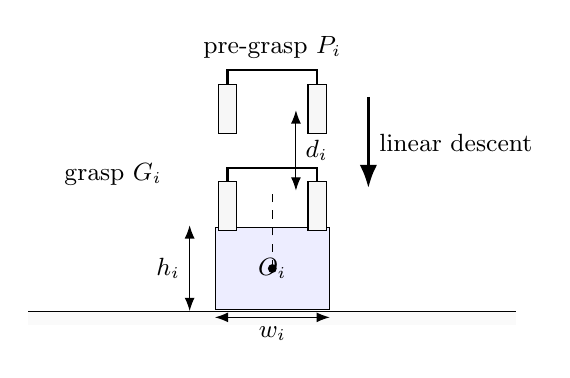
\begin{tikzpicture}[
  >=Latex,
  every node/.style={font=\small},
  block/.style={draw,fill=blue!7,minimum width=1.45cm,minimum height=1.05cm},
  finger/.style={draw,fill=gray!30,minimum width=0.16cm,minimum height=0.62cm}
]
  % Table and block
  \fill[gray!18] (-3.1,-0.08) rectangle (3.1,0.10);
  \draw (-3.1,0.10) -- (3.1,0.10);
  \node[block] (cube) at (0,0.64) {$O_i$};
  \draw[dashed] (0,0.64) -- (0,1.63);
  \fill (0,0.64) circle (1.6pt);

  % Final grasp
  \node[finger] at (-0.57,1.43) {};
  \node[finger] at (0.57,1.43) {};
  \draw[thick] (-0.57,1.74) -- (-0.57,1.92) -- (0.57,1.92)
    -- (0.57,1.74);
  \node[left] at (-1.28,1.83) {grasp $G_i$};

  % Pre-grasp
  \node[finger] at (-0.57,2.67) {};
  \node[finger] at (0.57,2.67) {};
  \draw[thick] (-0.57,2.98) -- (-0.57,3.16) -- (0.57,3.16)
    -- (0.57,2.98);
  \node[above] at (0,3.18) {pre-grasp $P_i$};
  \draw[->,very thick] (1.22,2.82) -- (1.22,1.66)
    node[midway,right] {linear descent};
  \draw[<->] (0.30,1.63) -- (0.30,2.65)
    node[midway,right] {$d_i$};

  % Dimensions
  \draw[<->] (-1.05,0.10) -- (-1.05,1.19)
    node[midway,left] {$h_i$};
  \draw[<->] (-0.73,0.02) -- (0.73,0.02)
    node[midway,below] {$w_i$};
\end{tikzpicture}
\caption{Top-grasp geometry. The TCP first moves to a pre-grasp pose above the
block and then follows a collision-checked linear Cartesian segment to the final
grasp. The object frame $O_i$, TCP frame $G_i$, and clearance $d_i$ must use the
same transform convention.}
\label{fig:grasp}
\end{figure}

\subsection{Algorithm and planner interface}

\Cref{alg:stack} separates global motion from contact-relevant motion. Joint-space
planning is suitable for the long move to the pre-grasp pose. The final approach
and withdrawal are short Cartesian segments, so their direction remains
vertical and their swept volume can be checked explicitly. The planner returns
a trajectory only if the complete path, including the attached block after a
grasp, is collision-free.

\begin{algorithm}[t]
\caption{Collision-aware block stacking}
\label{alg:stack}
\begin{algorithmic}[1]
\REQUIRE initial joint state $\mathbf{q}_0$, blocks $\{O_i\}$, table frame
\ENSURE ordered manipulation attempts
\STATE $\mathcal{S}\leftarrow\mathrm{BuildScene}(\{O_i\},\text{table})$
\STATE $\mathbf{q}\leftarrow\mathbf{q}_0$; order $\leftarrow\mathrm{StableOrder}(O_1,\ldots,O_N)$
\FOR{each block $i$ in order}
  \STATE $\mathbf{T}_{B\leftarrow G_i}\leftarrow
    \mathbf{T}_{B\leftarrow O_i}\mathbf{T}_{O_i\leftarrow G}$
  \STATE $\mathbf{T}_{B\leftarrow P_i}\leftarrow
    \mathbf{T}_{B\leftarrow G_i}\operatorname{Trans}(0,0,-d_i)$
\STATE $\tau_1\leftarrow\texttt{motion\_plan}
    (\mathbf{q},\mathbf{T}_{B\leftarrow P_i},\mathcal{S},\mathrm{constraints})$
  \IF{$\tau_1$ is not feasible}
    \STATE $\mathrm{TryFallbackGrasp}(i)$ \textbf{or continue}
  \ENDIF
  \STATE $\mathrm{Execute}(\tau_1)$
  \STATE $\tau_2\leftarrow\mathrm{LinearPlan}
    (\mathbf{T}_{B\leftarrow P_i},\mathbf{T}_{B\leftarrow G_i},\mathcal{S})$
  \STATE $\mathrm{CheckSweptVolume}(\tau_2)$; $\mathrm{Execute}(\tau_2)$
  \STATE $\mathrm{Open}(\mathbf{w}_i)$; $\mathrm{Execute}(\tau_2)$ end pose;
    $\mathrm{Close}(\mathbf{f}_i)$
  \STATE $\mathcal{S}\leftarrow\mathrm{Attach}(i,\mathrm{gripper})$
  \STATE $\mathbf{T}_{B\leftarrow L_i}\leftarrow
    \mathbf{T}_{B\leftarrow G_i}\operatorname{Trans}(0,0,l_{\mathrm{lift}})$
\STATE $\tau_3\leftarrow\texttt{motion\_plan}
    (\mathrm{current},\mathbf{T}_{B\leftarrow L_i},\mathcal{S},\mathrm{attached}=i)$
  \STATE $\mathrm{Execute}(\tau_3)$
  \STATE compute $\mathbf{T}_{B\leftarrow O_i^{*}}$ and
    $\mathbf{T}_{B\leftarrow G_i^{*}}$ with \cref{eq:placeheight,eq:placepose}
  \STATE plan and execute the collision-free transfer to the pre-place pose
  \STATE descend linearly, open the gripper, detach $i$, and add $i$ to
    $\mathcal{S}$ at its measured place pose
  \STATE retreat vertically and update $\mathbf{q}$
\ENDFOR
\end{algorithmic}
\end{algorithm}

\begin{table}[t]
\caption{Arguments expected by the planning interface. A library may name them
differently, but the information must be supplied in some form.}
\label{tab:api}
\centering
\small
\begin{tabularx}{\linewidth}{@{}lX@{}}
\toprule
Argument & Meaning and computation \\
\midrule
\texttt{start\_q} & Current joint vector from encoders or the preceding
trajectory; used directly by a joint-space planner. \\
\texttt{goal} & Either $\mathbf{T}_{B\leftarrow P_i}$ or a joint vector returned
by inverse kinematics. Pose goals also require a seed configuration and a
position/orientation tolerance. \\
\texttt{scene} & Robot model, table, unheld blocks, and the currently attached
block. Transform every collision geometry into frame $B$. \\
\texttt{constraints} & Joint limits, velocity and acceleration limits, allowed
contact set, collision margin, planning timeout, and multiple-solution policy. \\
\texttt{attached} & Object rigidly attached to the TCP. It moves with the robot,
is checked against the scene, and is removed from the static obstacle set. \\
\bottomrule
\end{tabularx}
\end{table}

For example, a library-neutral interface can be written as
\begin{center}
\small
\texttt{motion\_plan(start\_q, goal\_pose, robot, scene, constraints, attached)}
\end{center}
and should return a time-parameterised trajectory together with a feasibility
flag. The table below makes the origin of each argument explicit.

\subsection{Minimising grasp collisions}

Planning directly to $\mathbf{T}_{B\leftarrow G_i}$ can fail even when the
final gripper pose is theoretically collision-free. The approach path can sweep
the fingers or palm through the block, and a dense top grasp leaves little room
for a planner to rotate near the target. The proposed strategy is deliberately
simple:
\begin{enumerate}[leftmargin=1.3em,itemsep=2pt,topsep=2pt]
  \item Align the gripper with the block's top face and place it above the block.
  \item Open the jaws to $g_{\mathrm{open}}=w_i+2\epsilon$.
  \item Plan the arm to the pre-grasp pose, not to the final grasp.
  \item Descend along the tool axis while checking the complete swept volume.
  \item Close the jaws and lift vertically before any lateral transfer.
\end{enumerate}
The required clearance is
$d_i\geq l_{\mathrm{tool}}+h_i+\epsilon$. If the descent is infeasible, the
controller can increase $d_i$, try a $90^\circ$ yaw about the vertical axis when
the block permits it, or choose a different block. A grasp should be rejected
unless the approach segment, finger closure, and initial lift all pass collision
and joint-limit checks \citep{coleman2014moveit,sundaresan2023curobo}.

\section{Perception with a Depth Camera}\label{sec:perception}

The assumptions above remove the hardest perception problem: the controller
already knows every object pose. A depth camera is needed when object poses are
not known, are occluded, or change after the robot has planned a motion. The
extension is not merely a replacement for a coordinate lookup; it changes the
system into a closed-loop state estimator and controller.

\subsection{From pixels to robot-frame geometry}

Let $(u,v)$ be a pixel, $z$ its depth, and
$\mathbf{K}$ the camera intrinsic matrix. In camera frame $C$,
\begin{equation}\label{eq:backproject}
  \mathbf{p}_C
  =
  z\mathbf{K}^{-1}
  \begin{bmatrix}u&v&1\end{bmatrix}^{\mathsf T}
  =
  z
  \begin{bmatrix}
    (u-c_x)/f_x\\
    (v-c_y)/f_y\\
    1
  \end{bmatrix}.
\end{equation}
The point is moved into the robot frame with
$\mathbf{p}_B=\mathbf{T}_{B\leftarrow C}\mathbf{p}_C$. For a fixed camera this
transform is the camera extrinsic calibration. For a wrist-mounted camera,
$\mathbf{T}_{B\leftarrow C}$ includes the current robot pose and the fixed
hand-eye transform $\mathbf{T}_{E\leftarrow C}$:
\begin{equation}\label{eq:handeye}
  \mathbf{T}_{B\leftarrow C}
  =
  \mathrm{FK}(\mathbf{q})\mathbf{T}_{E\leftarrow C},
\end{equation}
where $E$ is the end-effector frame. Calibration error enters the geometry
directly, so it should be included in the pose uncertainty and motion margin.

\subsection{Perception and execution pipeline}

\begin{figure}[t]
\centering
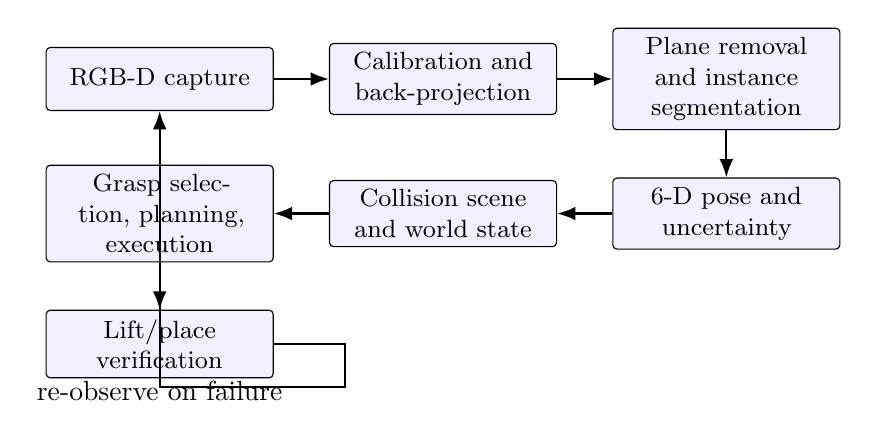
\begin{tikzpicture}[
  node distance=6mm and 7mm,
  box/.style={draw,rounded corners=1.5pt,fill=blue!6,align=center,
    minimum height=8mm,text width=2.65cm,font=\small},
  arrow/.style={->,>=Latex,thick}
]
  \node[box] (rgbd) {RGB-D capture};
  \node[box,right=of rgbd] (calib) {Calibration and back-projection};
  \node[box,right=of calib] (seg) {Plane removal and instance segmentation};
  \node[box,below=of seg] (pose) {6-D pose and uncertainty};
  \node[box,left=of pose] (scene) {Collision scene and world state};
  \node[box,left=of scene] (plan) {Grasp selection, planning, execution};
  \node[box,below=of plan] (verify) {Lift/place verification};

  \draw[arrow] (rgbd) -- (calib);
  \draw[arrow] (calib) -- (seg);
  \draw[arrow] (seg) -- (pose);
  \draw[arrow] (pose) -- (scene);
  \draw[arrow] (scene) -- (plan);
  \draw[arrow] (plan) -- (verify);
  \draw[arrow] (verify.east) -| ++(0.9,-0.55) -| (rgbd.south)
    node[pos=0.53,below] {re-observe on failure};
\end{tikzpicture}
\caption{A depth-camera extension. Perception is connected to execution by a
feedback loop: the robot re-observes after uncertain or failed grasps instead
of blindly executing a precomputed sequence.}
\label{fig:pipeline}
\end{figure}

The essential modules are:
\begin{enumerate}[leftmargin=1.3em,itemsep=2pt,topsep=2pt]
  \item \textbf{Calibration and filtering.} Estimate $\mathbf{K}$ and
    $\mathbf{T}_{B\leftarrow C}$, remove invalid depth pixels, and filter
    isolated points.
  \item \textbf{Segmentation.} Fit and remove the table plane with RANSAC
    \citep{fischler1981ransac}; divide the remaining point cloud into block
    instances using colour, geometric clusters, or an RGB instance mask.
  \item \textbf{Pose estimation.} Fit an oriented bounding box or register a
    known block model to the instance point cloud. ICP can refine the initial
    alignment when the object shape is known
    \citep{rusinkiewicz2001efficient}. Each estimate should include a covariance
    or a conservative uncertainty radius.
  \item \textbf{World-state update.} Insert only currently observed blocks into
    the collision scene, mark grasped blocks as attached, and inflate obstacle
    geometry by the pose uncertainty and planner margin.
  \item \textbf{Planning and control.} Generate grasp candidates from the latest
    pose estimates, plan to a pre-grasp, and re-observe near the object before
    the final approach.
  \item \textbf{Verification and recovery.} After lifting, verify that the block
    moved with the gripper. After placement, re-estimate its pose before
    releasing the task lock. If verification fails, retreat, re-observe, and
    replan.
\end{enumerate}
Point-cloud utilities such as Open3D provide filtering, segmentation, and
registration primitives for this pipeline \citep{zhou2018open3d}.

\subsection{Why the loop matters}

The planning stack described in \cref{sec:procedure} is intentionally
deterministic because the assignment grants exact object poses. That does not
make the complete system unintelligent: it shifts intelligence to where the
uncertainty is. The robot chooses a stack order, ranks feasible grasps, verifies
the result of each action, and changes its plan when perception or execution
contradicts the previous model.

Two engineering safeguards follow from this view. First, all estimates and
geometry should be expressed in a consistent frame; most apparently mysterious
robotics failures are frame-composition errors. Second, collision margins should
increase with pose uncertainty. A nominal centre that is 2\,mm from the support
edge is not safe when depth calibration has 5\,mm uncertainty. If the uncertainty
is too large, the correct action is to move to another viewpoint rather than to
compress the safety margin.

\begin{table}[t]
\caption{Representative perception failures and recovery actions.}
\label{tab:failure}
\centering
\small
\begin{tabularx}{\linewidth}{@{}lXX@{}}
\toprule
Failure & Detection & Recovery \\
\midrule
Occlusion & missing or partial instance mask &
move camera, choose another grasp, re-observe \\
Depth hole / reflection & sparse invalid region &
use RGB mask and model prior; reject unstable grasp \\
Incorrect pose & high registration residual or covariance &
re-segment, change viewpoint, inflate collision margin \\
Grasp slip & lift pose inconsistent with expected object motion &
stop transfer, lower safely, re-observe, retry \\
Placement offset & post-place block pose outside tolerance &
lift, reposition, or replan the remaining stack \\
\bottomrule
\end{tabularx}
\end{table}

\section{Discussion and Limitations}\label{sec:discussion}

The proposed baseline is deliberately modular. The known-pose version can be
implemented with any robot model, collision checker, and motion planner; the
depth-camera version adds perception without changing the meaning of the
planning interface. The design also exposes its assumptions: the top grasp is
feasible, the blocks are rigid, and a stable support polygon can be identified.
It does not model gripper compliance, contact mechanics, or object slippage. A
real system should therefore use force feedback, a guarded final approach, and
conservative acceleration limits. Because this is a written assignment rather
than a simulator study, the report makes no claim about a measured success rate,
cycle time, or collision rate.

\section{Conclusion}\label{sec:conclusion}

Block stacking combines a small task description with several coupled robotics
problems: frame composition, grasp geometry, collision-aware motion generation,
stable placement, and perception under uncertainty. For the known-pose case,
the key idea is to plan to a safe pre-grasp, descend vertically, and attach the
object to the robot only after a successful grasp. For the depth-camera case,
the key idea is to turn perception into continuous state estimation and use it
to replan after uncertainty or failure. These feedback and safety checks make
the procedure more than a fixed sequence of motions.

\begingroup
\small
\setlength{\bibsep}{2pt}
\bibliographystyle{plainnat}
\bibliography{reference}
\endgroup

\end{document}
